\documentclass[11pt,a4paper]{article}
\usepackage[T1]{fontenc}
\usepackage[utf8]{inputenc}
\usepackage{lmodern,microtype}
\usepackage[margin=25mm,headheight=15pt]{geometry}
\usepackage{amsmath,amssymb,amsthm,mathtools,bm}
\usepackage{booktabs,tabularx,longtable,array}
\usepackage{graphicx,enumitem,fancyhdr,xurl}
\usepackage[dvipsnames]{xcolor}
\usepackage[colorlinks=true,linkcolor=MidnightBlue,citecolor=MidnightBlue,urlcolor=MidnightBlue]{hyperref}
\usepackage[nameinlink,noabbrev]{cleveref}
\hypersetup{pdftitle={Elliptic Equilibrium and Boundary-Corrected Transseries for Hyperbolic Fekete Designs},pdfauthor={Research manuscript prepared for Vladimir Reshetnikov},pdfsubject={Fabius common-digit covariance, elliptic equilibrium, screened energy, and determinant asymptotics}}
\pagestyle{fancy}\fancyhf{}
\fancyhead[L]{\small Elliptic equilibrium and hyperbolic Fekete designs}
\fancyhead[R]{\small Research manuscript}
\fancyfoot[C]{\thepage}
\setlength{\emergencystretch}{2em}
\allowdisplaybreaks
\newtheorem{theorem}{Theorem}[section]
\newtheorem{lemma}[theorem]{Lemma}
\newtheorem{proposition}[theorem]{Proposition}
\newtheorem{corollary}[theorem]{Corollary}
\theoremstyle{definition}
\newtheorem{definition}[theorem]{Definition}
\newtheorem{question}[theorem]{Research question}
\theoremstyle{remark}
\newtheorem{remark}[theorem]{Remark}
\newcommand{\R}{\mathbb R}
\newcommand{\N}{\mathbb N}
\newcommand{\dd}{\,\mathrm d}
\newcommand{\sech}{\operatorname{sech}}
\newcommand{\PV}{\operatorname{PV}}
\newcommand{\diag}{\operatorname{diag}}
\newcommand{\supp}{\operatorname{supp}}
\newcommand{\E}{\mathcal E}
\newcommand{\Dopt}{\mathcal D}
\newcommand{\cC}{\mathcal C}
\newcommand{\ones}{\mathbf 1}
\newcommand{\norm}[1]{\left\lVert#1\right\rVert}
\newcommand{\abs}[1]{\left\lvert#1\right\rvert}
\newcommand{\poc}[1]{\left(#1;#1\right)_\infty}
\newcommand{\K}{\mathrm K}
\newcommand{\repoid}{\texttt{0c973d8f5e7ef4550f4df1bf486d890037fd9f14}}

\begin{document}
% ed. (2026-09-29): no page anchors on the title page, which removes the
% duplicate hyperref destination page.1 (pdfTeX warning).
\hypersetup{pageanchor=false}
\begin{titlepage}
\vspace*{12mm}
\noindent{\small\scshape ProveIt research continuation \hfill 29 September 2026}
\vspace{16mm}
\begin{flushleft}
{\Huge\bfseries Elliptic Equilibrium and\par Boundary-Corrected Transseries\par for Hyperbolic Fekete Designs\par}
\vspace{9mm}
{\Large An explicit Fabius design limit, screened crystallization,\par and a finite-size determinant transition\par}
\vspace{11mm}
{\large Research manuscript prepared for Vladimir Reshetnikov}
\end{flushleft}
\vspace{12mm}
\begin{abstract}
The common-digit Fabius construction in the ProveIt repository leads to the
covariance kernel $\sech(u-v)$ and asks for the limiting distribution of
parameters maximizing its determinant on a fixed interval. We solve the
equilibrium-measure part of that question explicitly. The density is an
elliptic deformation of the arcsine law, its constant potential is a ratio
of complete elliptic integrals, and its large-interval expansion admits a
convergent exponential--logarithmic representation with a certified inverse.
These continuum results are connected with classical Green capacity rather
than presented as a new discovery of elliptic capacity.

The finite-design analysis goes further. We prove explicit two-sided energy
bounds, a dimension-independent bound on deviations from equal spacing when
the mean gap stays positive, and a dimension-uniform dilute boundary
correction. The latter quantifies the failure of the equally spaced design:
its energy exceeds the optimum by
$2(n-3)e^{-6h}/(n-1)+O(e^{-8h})$, with an absolute remainder uniform in the
number of nodes. It yields a deterministic transition
$\det R_n^*\to\exp(-4e^{-2s})$ at
$h=\tfrac12\log n+s$, together with three finite-size correction orders.
Exact $q$-product factorizations and a modular bulk expansion provide the
transseries connection. Full proofs, reproducible numerical diagnostics,
source provenance, and further research questions are included. Microscopic
fixed-interval endpoint spacings and a complete joint MacMahon asymptotic
are explicitly left open.
\end{abstract}
\vfill
\noindent\textbf{Status.} A mathematical research manuscript with proofs and numerical
checks, not a Lean formalization or an independently refereed paper. Claims
of worldwide priority are not made. The main new-development target is the
uniform finite-design boundary analysis, not the classical elliptic formulas.
\end{titlepage}
\hypersetup{pageanchor=true}

\setcounter{tocdepth}{1}
\tableofcontents
\newpage

\section{Problem, provenance, and scope}
\label{sec:scope}

\subsection{The precise repository question}
The starting point is the repository report \emph{Common-Digit Fabius Zonoids:
Exact volumes, hyperbolic-secant geometry, Bernoulli Gaussianization, and
parameter jets}~\cite{repo}. Its section on hyperbolic node design proves the
existence and uniqueness of a configuration maximizing
\begin{equation}
 \prod_{1\le i<j\le n}\tanh(u_j-u_i),
 \qquad 0\le u_1<\cdots<u_n\le L.
 \label{eq:product}
\end{equation}
The later question labeled \texttt{question:design-limit} asks for the limiting
empirical measure, an explicit constant-potential density, and endpoint
spacings. The question labeled \texttt{question:q-barnes} asks for joint
asymptotics and modular transseries of the equally spaced product.

The source was inspected at the repository commit
\begin{center}\small\repoid.\end{center}
The relevant file has Git blob identifier
\texttt{dabfc501dfe952d826001703a087b47424568581}. Its exact path and the
inspected source ranges are recorded in \cref{sec:provenance} and in the
archive's \texttt{PROVENANCE.md}. The present paper does not infer that a
statement in that research report is machine-checked. The covariance and
determinant facts needed here are rederived below.

\subsection{Normalization}
Throughout, logarithms are natural. Set
\begin{equation}
 V(x)=-\log\tanh x\quad(x>0),\qquad V(0)=+\infty,
 \qquad
 E_n(u)=\sum_{i<j}V(u_j-u_i).
 \label{eq:energy}
\end{equation}
The minimum on the interval is denoted by $E_n^*(L)$. We use
\begin{equation}
 P_n^*(L)=e^{-E_n^*(L)},\qquad
 \Dopt_n(L)=e^{-2E_n^*(L)}.
 \label{eq:PD}
\end{equation}
Thus $P_n^*$ is the optimal product in \eqref{eq:product}, while $\Dopt_n$ is
the optimal covariance determinant. This factor of two is kept explicit.
For a probability measure $\mu$ on $[0,L]$, define
\begin{equation}
 \E_L(\mu)=\iint V(|u-v|)\dd\mu(u)\dd\mu(v).
 \label{eq:continuumenergy}
\end{equation}
The notation $\K(k)$ always uses the \emph{elliptic modulus}:
\begin{equation}
 \K(k)=\int_0^{\pi/2}\frac{\dd\theta}{\sqrt{1-k^2\sin^2\theta}}.
 \label{eq:Kdef}
\end{equation}
Software interfaces using the parameter $m=k^2$ must be supplied with $k^2$,
not with $k$.

\subsection{What is established here}
The continuum question is answered by
\begin{equation}
 \boxed{\displaystyle
 \rho_L(u)=\frac{2}{\K(k)
 \sqrt{(1-e^{-4u})(1-e^{-4(L-u)})}},\qquad
 k=\sqrt{1-e^{-4L}}.}
 \label{eq:main-density}
\end{equation}
Its equilibrium energy is
\begin{equation}
 \boxed{\displaystyle I_L=\pi\frac{\K(e^{-2L})}{\K(\sqrt{1-e^{-4L}})}.}
 \label{eq:main-I}
\end{equation}
Every sequence of optimal empirical measures converges to $\rho_L(u)\dd u$
for fixed $L$, and $\log\Dopt_n(L)/(n(n-1))\to-I_L$.

For the discrete problem put $m=n-1$, $h=L/m$, and $q=e^{-2h}$. With
\begin{equation}
 U_n(h)=\sum_{k=1}^{n-1}(n-k)V(kh),
 \label{eq:gridenergy}
\end{equation}
we prove the dimension-uniform formula
\begin{equation}
 \boxed{\displaystyle
 E_n^*((n-1)h)=U_n(h)-2\frac{n-3}{n-1}q^3+O(q^4),\qquad n\ge3.}
 \label{eq:mainboundary}
\end{equation}
The constant in $O(q^4)$ is independent of $n$. Consequently, at
$h=\tfrac12\log n+s$,
\begin{equation}
 \boxed{\displaystyle
 \Dopt_n((n-1)h)\longrightarrow \exp(-4e^{-2s}).}
 \label{eq:maintransition}
\end{equation}
A three-order correction to the energy is proved in \cref{thm:critical}.
The uniformity in \eqref{eq:mainboundary}, rather than a fixed-$n$ Taylor
series, is what permits this growing-dimensional substitution.

\subsection{Classical ingredients and novelty boundary}
Green equilibrium, transfinite diameter, and convergence of minimizing
configurations are classical themes; Saff's account~\cite{saff} provides
background. The elliptic modulus of a disk slit by a geodesic segment is
also classical. In particular, the capacity discussion in
Nasser--Rainio--Vuorinen~\cite{nrv} identifies the corresponding
Gr\"otzsch elliptic ratio. We give an elementary derivation in the precise
coordinates of the repository problem. The elliptic and eta expansions
used later are standard formulas recorded by NIST~\cite{dlmf19,dlmf23}.

The contributions developed specifically in this manuscript are the
quantitative finite-design estimates, the bounded total gap-defect theorem,
and especially the absolute, dimension-uniform boundary correction and its
finite-size transition consequences. A targeted literature check did not
establish a published match for that particular package of statements.
That is not a proof of priority; the theorems are offered with proofs, not
with an unsupported claim to settle a famous general Fekete problem.

\section{From common digits to a strictly convex design problem}
\label{sec:covariance}

\subsection{A direct covariance calculation}
Let $U_0,U_1,\ldots$ be independent uniform random variables on $[0,1]$, and
for $0\le r<1$ set
\begin{equation}
 X_r=(1-r)\sum_{j\ge0}r^jU_j.
 \label{eq:Xr}
\end{equation}
The series converges absolutely for every sample. Independence gives
\begin{align}
 \operatorname{Var}(X_r)&=\frac{1-r}{12(1+r)},\label{eq:variance}\\
 \operatorname{Cov}(X_r,X_t)&=\frac{(1-r)(1-t)}{12(1-rt)}.
 \label{eq:cov}
\end{align}
After standardization and the substitutions $r=\tanh u$, $t=\tanh v$,
\begin{equation}
 \operatorname{Corr}(X_{\tanh u},X_{\tanh v})
 =\frac{\sqrt{(1-r^2)(1-t^2)}}{1-rt}=\sech(u-v).
 \label{eq:sech-cov}
\end{equation}
This is the common-digit covariance connection in the repository report.
It is an exact identity, not a Gaussian approximation.

\begin{proposition}[Cauchy determinant identity]
\label{prop:det}
For distinct real $u_1,\ldots,u_n$, the matrix
$R(u)=[\sech(u_i-u_j)]_{i,j=1}^n$ satisfies
\begin{equation}
 \det R(u)=\prod_{i<j}\tanh^2(u_j-u_i)=e^{-2E_n(u)}.
 \label{eq:detidentity}
\end{equation}
\end{proposition}
\begin{proof}
Put $t_i=e^{2u_i}$. Then
$R_{ij}=2\sqrt{t_it_j}/(t_i+t_j)$. The Cauchy determinant formula gives
\[
 \det\left[\frac1{t_i+t_j}\right]
 =\frac{\prod_{i<j}(t_j-t_i)^2}{\prod_{i,j}(t_i+t_j)}.
\]
Multiplication by the row and column factors contributes $\prod_i2t_i$,
which cancels the diagonal factors in the denominator. The remaining
factor for each pair is $((t_j-t_i)/(t_j+t_i))^2$, as required.
\end{proof}

\subsection{The interaction and the optimizer}
For $x>0$, elementary differentiation and the power series for the logarithm
give
\begin{align}
 V(x)&=2\sum_{\substack{r\ge1\\r\ \mathrm{odd}}}\frac{e^{-2rx}}r,
 \label{eq:Vseries}\\
 V'(x)&=-\frac2{\sinh(2x)},\qquad
 V''(x)=\frac{4\cosh(2x)}{\sinh^2(2x)}>0.
 \label{eq:Vderiv}
\end{align}
Thus $V$ is positive, decreasing, strictly convex, logarithmically singular
at zero, and exponentially decreasing at infinity.

\begin{proposition}[Unique finite optimizer]
\label{prop:unique}
For $n\ge2$ and $L>0$, the minimizing configuration exists and is unique
among ordered configurations. It has $u_1=0$, $u_n=L$, and
$u_i+u_{n+1-i}=L$. Its interior nodes satisfy
\begin{equation}
 \sum_{j<i}V'(u_i-u_j)-\sum_{j>i}V'(u_j-u_i)=0,
 \qquad 2\le i\le n-1.
 \label{eq:stationarity}
\end{equation}
\end{proposition}
\begin{proof}
Extend the energy by $+\infty$ at collisions. Lower semicontinuity on the
compact ordered simplex gives a minimum; a strictly ordered test
configuration has finite energy, so a minimizer has no collision. The
leftmost point must be zero: moving it to zero strictly increases all its
distances if it was positive and hence decreases the energy. The same
argument applies to the rightmost point.

Write the positive gaps as $d_i=u_{i+1}-u_i$, $1\le i\le m=n-1$, with
$\sum_i d_i=L$. Each summand of the energy is a convex function of a sum of
consecutive gaps. The nearest-neighbor contribution $\sum_iV(d_i)$ is
strictly convex. Hence the whole energy is strictly convex on this affine
simplex. This proves uniqueness. Reflection preserves the objective, so
uniqueness implies the symmetry. Differentiating at the interior minimizer
gives \eqref{eq:stationarity}.
\end{proof}

For $n=2,3$ the equally spaced design is optimal. For larger $n$ it is not
generally optimal, despite becoming an accurate approximation in dilute
regimes. The size and structure of that difference are quantified below.

\section{Exact elliptic equilibrium on a fixed interval}
\label{sec:equilibrium}

\subsection{A useful change of variables}
Let
\begin{equation}
 b=e^{2L},\qquad k=\sqrt{1-b^{-2}},\qquad k'=b^{-1}.
 \label{eq:moduli}
\end{equation}
Under $t=e^{2u}$ and $s=e^{2v}$,
\begin{equation}
 V(|u-v|)=\log\left|\frac{t+s}{t-s}\right|,
 \qquad 1\le t,s\le b.
 \label{eq:green-kernel}
\end{equation}
The candidate density in these variables is
\begin{equation}
 w_b(t)=\frac{b}{\K(k)\sqrt{(t^2-1)(b^2-t^2)}},\qquad 1<t<b.
 \label{eq:w}
\end{equation}
Indeed,
\begin{equation}
 \int_1^b\frac{\dd t}{\sqrt{(t^2-1)(b^2-t^2)}}=\frac{\K(k)}b.
 \label{eq:normelliptic}
\end{equation}
For example, substitute $t^2=1+(b^2-1)\sin^2\theta$; the left side becomes
$\int_0^{\pi/2}(1+(b^2-1)\sin^2\theta)^{-1/2}\dd\theta$.
Changing $\theta$ to $\pi/2-\theta$ factors out $b^{-1}$ and gives
\eqref{eq:normelliptic}.

\begin{lemma}[An arcsine Cauchy integral]
\label{lem:arcsine}
For $A<B$,
\begin{equation}
 \int_A^B\frac{\dd y}{(y-z)\sqrt{(y-A)(B-y)}}
 =\frac{\pi}{\sqrt{(A-z)(B-z)}}\quad(z<A),
 \label{eq:arcsineoutside}
\end{equation}
where the square roots on the right are positive. For $A<z<B$ the
principal value of the same integral is zero.
\end{lemma}
\begin{proof}
The affine cosine substitution $y=(A+B)/2+(B-A)\cos\theta/2$ reduces the
first identity to the elementary integral
$\int_0^\pi(c+d\cos\theta)^{-1}\dd\theta=\pi/\sqrt{c^2-d^2}$ for $c>|d|$.
It follows by $\tan(\theta/2)$ substitution. The same substitution in the
principal-value case gives the principal value of
$\int_0^\infty(\alpha-\beta x^2)^{-1}\dd x$ for $\alpha,\beta>0$.
Its logarithmic antiderivative has equal limits at zero and infinity, and
the two logarithmic divergences at its pole cancel. Its principal value is
therefore zero.
\end{proof}

\begin{theorem}[Explicit equilibrium measure and potential]
\label{thm:equilibrium}
The density $\rho_L$ in \eqref{eq:main-density} is a probability density on
$(0,L)$. Its potential is constant on the whole closed interval:
\begin{equation}
 \int_0^L V(|u-v|)\rho_L(v)\dd v
 =I_L=\pi\frac{\K(k')}{\K(k)},\qquad 0\le u\le L.
 \label{eq:constantpotential}
\end{equation}
It is the unique probability measure minimizing $\E_L$.
\end{theorem}
\begin{proof}
\emph{Normalization and change of density.}
Equation \eqref{eq:normelliptic} normalizes \eqref{eq:w}. Multiplication by
$\dd t/\dd u=2e^{2u}$ and factoring the two square roots gives exactly
\eqref{eq:main-density}.

\emph{Constancy in the interior.}
Let
\[
 W(t)=\int_1^b\log\left|\frac{t+s}{t-s}\right|w_b(s)\dd s.
\]
On every compact subinterval of $(1,b)$ the density is smooth, and
logarithmic-potential differentiation is given by a principal value.
This can also be proved directly by subtracting the density's value at
$s=t$ in the local singular integral; the subtracted numerator is
$O(s-t)$ and is integrable after differentiation. Thus
\begin{align*}
 W'(t)
 &=-\frac{2b}{\K(k)}\PV\int_1^b
 \frac{s\dd s}{(t^2-s^2)\sqrt{(s^2-1)(b^2-s^2)}}\\
 &=-\frac b{\K(k)}\PV\int_1^{b^2}
 \frac{\dd y}{(t^2-y)\sqrt{(y-1)(b^2-y)}}=0,
\end{align*}
by \cref{lem:arcsine}. Consequently $W$ is constant on $(1,b)$.
The square-root edge behavior of $w_b$ makes its logarithmic potential
continuous up to both endpoints. For completeness, the contribution of
an endpoint interval of length $\varepsilon$ is bounded by a constant
multiple of $\sqrt\varepsilon(1+|\log\varepsilon|)$; away from that interval
ordinary dominated convergence applies.

\emph{Evaluation of the constant.}
For $0\le t<1$ the logarithm is nonsingular and $W(0)=0$. Differentiating
and applying \eqref{eq:arcsineoutside} yields
\[
 W'(t)=\frac{b\pi}{\K(k)\sqrt{(1-t^2)(b^2-t^2)}}.
\]
Integration from zero to one, followed by $t=\sin\theta$, gives
$W(1)=\pi\K(1/b)/\K(k)$. Endpoint continuity identifies this with the
constant on the support.

\emph{Minimality and uniqueness.}
Let $\mu$ denote the measure just constructed. If a competing probability
measure $\nu$ has infinite energy, there is nothing to prove. Otherwise,
constant potential gives
$\iint V(|u-v|)\dd\mu(u)\dd\nu(v)=I_L$. For the signed measure
$\sigma=\nu-\mu$, all required integrals are absolutely defined, since
$|\sigma|\le\mu+\nu$. Hence
\begin{equation}
 \E_L(\nu)-I_L=\iint V(|u-v|)\dd\sigma(u)\dd\sigma(v).
 \label{eq:energy-difference}
\end{equation}
Every kernel $e^{-a|u-v|}$, $a>0$, is strictly positive definite on finite
signed measures. In the Fourier convention
$\widehat\sigma(\xi)=\int e^{-i\xi u}\dd\sigma(u)$,
\begin{equation}
 \iint e^{-a|u-v|}\dd\sigma(u)\dd\sigma(v)
 =\frac1{2\pi}\int_\R\frac{2a}{a^2+\xi^2}
 |\widehat\sigma(\xi)|^2\dd\xi\ge0.
 \label{eq:positivekernel}
\end{equation}
Fourier inversion is justified because $2a/(a^2+\xi^2)$ is integrable.
Equality implies $\widehat\sigma=0$ and therefore $\sigma=0$.
Expanding $V$ by \eqref{eq:Vseries} in \eqref{eq:energy-difference} is valid
by absolute integrability against $|\sigma|\otimes|\sigma|$. Every term is
nonnegative, and already the $r=1$ term is strictly positive unless
$\sigma=0$. This proves the assertion.
\end{proof}

\begin{remark}[Relation to classical capacity]
The map $r=\tanh u$ changes \eqref{eq:green-kernel} into the unit-disk Green
kernel $\log|(1-rt)/(r-t)|$ on a real segment. The classical Gr\"otzsch
expression for the same energy is
\begin{equation}
 I_L=\frac\pi2\frac{\K(\sech L)}{\K(\tanh L)}.
 \label{eq:groetzsch}
\end{equation}
The equivalence with \eqref{eq:main-I} is an elliptic Landen transformation.
With the convention that condenser capacity is $2\pi$ divided by the
minimum of this Green energy, it is $2\pi/I_L$. The formulas in
\cite{nrv} supply the classical capacity interpretation. Our derivation
of \cref{thm:equilibrium} does not require the conformal mapping theorem or
an imported formula for the equilibrium density.
\end{remark}

\section{Discrete convergence and the two continuum edge regimes}
\label{sec:convergence}

\begin{theorem}[Convergence of optimal designs]
\label{thm:convergence}
For fixed $L>0$, let $u^{(n)}$ minimize $E_n$ and set
$\mu_n=n^{-1}\sum_{i=1}^n\delta_{u_i^{(n)}}$. Then
\begin{equation}
 \mu_n\Rightarrow\mu_L=\rho_L(u)\dd u,
 \qquad
 \frac{2E_n^*(L)}{n(n-1)}\longrightarrow I_L.
 \label{eq:weakconvergence}
\end{equation}
In particular,
\begin{equation}
 (P_n^*(L))^{2/(n(n-1))}\longrightarrow e^{-I_L},\qquad
 \Dopt_n(L)^{1/(n(n-1))}\longrightarrow e^{-I_L}.
 \label{eq:capacitylimits}
\end{equation}
\end{theorem}
\begin{proof}
Choose $n$ independent points with distribution $\mu_L$. Their expected
energy is $n(n-1)I_L/2$. Some configuration has energy no larger than this
expectation, so $2E_n^*(L)/(n(n-1))\le I_L$.

For the converse, put $V_M(x)=\min(V(x),M)$, with $V_M(0)=M$. It is bounded
and continuous. Along any weakly convergent subsequence $\mu_n\Rightarrow\nu$,
\[
 \iint V_M(|u-v|)\dd\mu_n(u)\dd\mu_n(v)
 \le\frac{2E_n^*(L)}{n^2}+\frac Mn.
\]
Weak convergence of product measures gives the corresponding limiting
inequality for $\nu$. Letting $M\to\infty$ and using monotone convergence,
\[
 I_L\le\E_L(\nu)\le\liminf_n\frac{2E_n^*(L)}{n^2}\le I_L.
\]
Uniqueness in \cref{thm:equilibrium} forces $\nu=\mu_L$. Compactness of
probability measures on $[0,L]$ now shows that the full sequence converges.
The product and determinant statements follow from \eqref{eq:PD}.
\end{proof}

\subsection{What the density says at an endpoint}
\begin{proposition}[Continuum edge and quantile scales]
\label{prop:edges}
For fixed $L>0$,
\begin{equation}
 \rho_L(u)=\frac{1+O(u)}{k\K(k)\sqrt u},\qquad u\downarrow0,
 \label{eq:edge-density}
\end{equation}
and the right endpoint has the reflected expansion. If $Q_L(p)$ is the
quantile of $\mu_L$, then
\begin{equation}
 Q_L(p)=\frac{(k\K(k))^2}{4}p^2(1+O(p^2)),\qquad p\downarrow0.
 \label{eq:edge-quantile}
\end{equation}
\end{proposition}
\begin{proof}
Expand $1-e^{-4u}=4u(1+O(u))$ and
$1-e^{-4(L-u)}=k^2(1+O(u))$ in \eqref{eq:main-density}. Integration gives
$\mu_L([0,u])=2\sqrt u/(k\K(k))(1+O(u))$. Inverting this expression yields
\eqref{eq:edge-quantile}.
\end{proof}

\textbf{Important distinction.} Formula \eqref{eq:edge-quantile} is a
continuum statement. Weak convergence in \cref{thm:convergence} does not
justify inserting $p=1/n$ to obtain the first discrete gap. Such a claim
would require a microscopic theorem not proved here. This is precisely the
part of the repository's endpoint-spacing question that remains open.

\subsection{Short intervals and screened long intervals}
\begin{proposition}[Arcsine limit, bulk flattening, and surface excess]
\label{prop:continuumregimes}
As $L\downarrow0$, the rescaled measures converge in total variation to the
arcsine law:
\begin{equation}
 L\rho_L(Lx)\longrightarrow\frac1{\pi\sqrt{x(1-x)}}
 \quad\text{in }L^1(0,1).
 \label{eq:arcsine-limit}
\end{equation}
As $L\to\infty$, put $\ell=L+\log2$. For fixed $u>0$,
\begin{equation}
 \ell\rho_L(u)\longrightarrow(1-e^{-4u})^{-1/2}.
 \label{eq:boundarylayer}
\end{equation}
Uniformly where $u$ and $L-u$ both tend to infinity,
$\ell\rho_L(u)\to1$. The single-edge excess of the limiting boundary layer is
\begin{equation}
 \int_0^\infty\left((1-e^{-4u})^{-1/2}-1\right)\dd u
 =\frac{\log2}{2}.
 \label{eq:surfaceexcess}
\end{equation}
\end{proposition}
\begin{proof}
For the short-interval limit, $k\to0$ and $\K(k)\to\pi/2$.
The two factors in the square root of \eqref{eq:main-density} are
$4Lx(1+O(L))$ and $4L(1-x)(1+O(L))$, uniformly for $0<x<1$ in the relative
sense. The rescaled densities are bounded by a fixed multiple of
$[x(1-x)]^{-1/2}$, so dominated convergence proves \eqref{eq:arcsine-limit}.

For the long-interval limit, the elliptic expansion proved in the next
section gives $\K(k)=2\ell+O(Le^{-4L})$. Substitute this into the exact
density to obtain \eqref{eq:boundarylayer} and the bulk statement.
Finally, $y=e^{-4u}$ transforms \eqref{eq:surfaceexcess} into
\[
 \frac14\int_0^1\frac{(1-y)^{-1/2}-1}{y}\dd y.
\]
With $t=\sqrt{1-y}$ this equals
$\frac12\int_0^1(1+t)^{-1}\dd t=\frac12\log2$.
\end{proof}

The effective length $L+\log2$ therefore has a geometric interpretation:
the two edges each supply excess mass corresponding to half of $\log2$.
The arcsine edge singularity survives while the interior becomes nearly
flat. This makes precise the qualitative prediction in the repository.

\begin{figure}[tb]
 \centering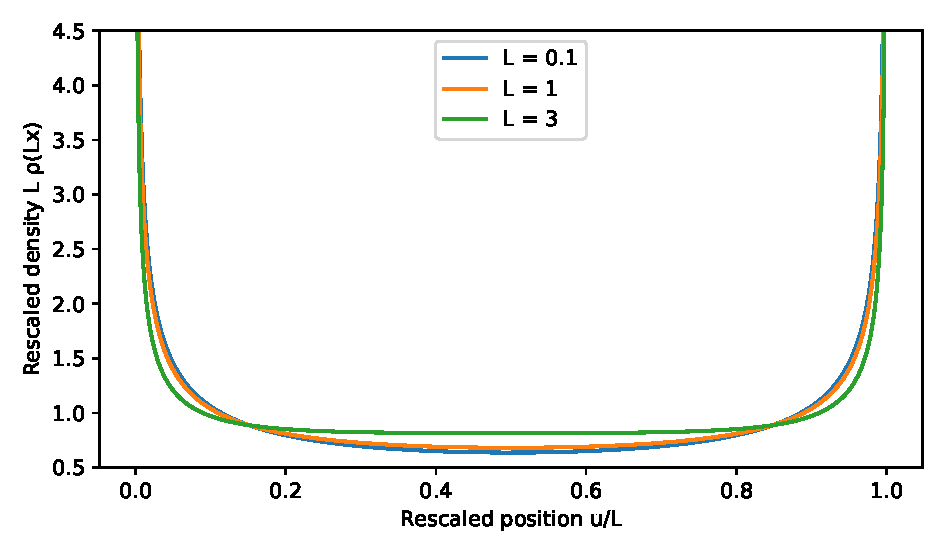
\includegraphics[width=.88\textwidth]{verification/equilibrium_density.pdf}
 \caption{The exact rescaled equilibrium density. Short intervals approach
 the arcsine profile; longer intervals have a flatter interior and thinner
 boundary layers. The vertical axis is truncated only for legibility.}
 \label{fig:density}
\end{figure}

\section{Convergent capacity transseries and certified inversion}
\label{sec:capacity-transseries}

\subsection{A convergent exponential--logarithmic normal form}
Let $z=e^{-4L}$, $H=\log(4e^{2L})=2L+2\log2$, and define
\begin{align}
 a_j&=\left(\frac{(1/2)_j}{j!}\right)^2,\qquad
 d_j=2(H_{2j}-H_j),\qquad d_0=0,\label{eq:ad}\\
 A(z)&=\sum_{j\ge0}a_jz^j,\qquad
 D(z)=\sum_{j\ge1}a_jd_jz^j,\qquad B(z)=D(z)/A(z).
 \label{eq:ADB}
\end{align}
Here $H_j=\sum_{r=1}^j1/r$ is a harmonic number, with $H_0=0$.
The convergent complete-elliptic-integral expansions in
NIST~\cite[\S19.12]{dlmf19} give
\begin{equation}
 \K(\sqrt z)=\frac\pi2 A(z),\qquad
 \K(\sqrt{1-z})=H A(z)-D(z).
 \label{eq:Kseries}
\end{equation}
The $\log4$ in $H$ absorbs the $j=0$ digamma constant in the usual formula.

\begin{theorem}[Capacity expansion with a positive error certificate]
\label{thm:capacity-series}
For every $L>0$,
\begin{equation}
 I_L=\frac{\pi^2}{2(H-B(z))}
 =\frac{\pi^2}{4(L+\log2-B(e^{-4L})/2)}.
 \label{eq:I-normalform}
\end{equation}
The Taylor series of $B$ converges for $|z|<1$ and begins
\begin{equation}
 B(z)=\frac z4+\frac{13z^2}{128}+\frac{23z^3}{384}
 +\frac{2701z^4}{65536}+\frac{5057z^5}{163840}+O(z^6).
 \label{eq:Bcoeff}
\end{equation}
Let $A_N,D_N$ be the truncations through degree $N$, and put
\begin{equation}
 I_{L,N}=\frac{\pi^2}{2(H-D_N(z)/A_N(z))}.
 \label{eq:Iapprox}
\end{equation}
Then
\begin{equation}
 0\le I_L-I_{L,N}
 \le\frac{\pi^2\log2}{4L^2}\frac{z^{N+1}}{1-z}.
 \label{eq:Icertificate}
\end{equation}
\end{theorem}
\begin{proof}
The normal form follows by dividing the two expressions in
\eqref{eq:Kseries}. The functions $A,D$ are analytic on $|z|<1$.
Moreover,
\[
 A(z)=\frac2\pi\int_0^{\pi/2}(1-z\sin^2\theta)^{-1/2}\dd\theta
\]
has positive real part there: $1-z\sin^2\theta$ has positive real part,
and so does its principal inverse square root. Thus $A$ has no zero in
the unit disk, proving analyticity of $B$. The coefficients in
\eqref{eq:Bcoeff} follow by ordinary power-series division.

For real $0<z<1$, $0<a_j\le1$, and $d_j$ increases from zero to $2\log2$.
Consequently $D/A$ is a weighted average of the $d_j$, and adding its tail
can only increase the average. In detail,
\[
 0\le B(z)-\frac{D_N(z)}{A_N(z)}
 \le 2\log2\sum_{j>N}a_jz^j
 \le 2\log2\frac{z^{N+1}}{1-z}.
\]
Both $H-B$ and $H-D_N/A_N$ are at least $H-2\log2=2L$.
Subtracting the two reciprocals in \eqref{eq:I-normalform} and
\eqref{eq:Iapprox} gives \eqref{eq:Icertificate}.
\end{proof}

For example, with $\ell=L+\log2$,
\begin{equation}
 I_L=\frac{\pi^2}{4\ell}
 \left[1+\frac{e^{-4L}}{8\ell}
 +\left(\frac{13}{256\ell}+\frac1{64\ell^2}\right)e^{-8L}
 +O\!\left(\frac{e^{-12L}}\ell\right)\right]
 \label{eq:I-firstsectors}
\end{equation}
as $L\to\infty$. More generally, $(H-B)^{-1}=\sum_{r\ge0}B^r/H^{r+1}$ is a convergent
expansion in the analytic block $B(z)$ for every real $L>0$, since
$0\le B<2\log2<H$. Expanding the blocks into exponential sectors yields
an absolutely convergent exponential--logarithmic series for sufficiently
large $L$: then the absolutely summed Taylor coefficients of $B$ are
smaller than $H$.
It is not necessary to invoke Borel summation or resurgence for this
particular expansion.

\subsection{Inverse interval design and exponentially invisible corrections}
For a prescribed small equilibrium energy $I>0$, one may ask for the
interval length $L$ producing it. This connects the equilibrium result
directly with the repository's inversion program.

\begin{theorem}[A certified inverse-capacity transseries]
\label{thm:inverse-capacity}
The map $L\mapsto I_L$ is continuous and strictly decreasing from $+\infty$
to zero. Write its inverse as $L=L(I)$. Set
\begin{equation}
 X=\frac{\pi^2}{4I},\qquad Q=e^{-\pi^2/I},\qquad\varepsilon=16Q.
 \label{eq:inverseparameters}
\end{equation}
For $16Q<1/64$, there is an analytic function $w(\varepsilon)$ at zero such that
\begin{equation}
 L(I)=X-\log2+w(\varepsilon),\qquad
 w=\frac12B(\varepsilon e^{-4w}).
 \label{eq:inversefixedpoint}
\end{equation}
Its coefficients have the nonrecursive formula
\begin{equation}
 [\varepsilon^j]w(\varepsilon)
 =\frac1{2j}[t^{j-1}]B'(t)e^{-2jB(t)},\qquad j\ge1.
 \label{eq:inversecoeff}
\end{equation}
In particular,
\begin{align}
 L(I)={}&\frac{\pi^2}{4I}-\log2+2Q-3Q^2+\frac83Q^3
 -\frac32Q^4+\frac{12}{5}Q^5+O(Q^6).
 \label{eq:inverseexpansion}
\end{align}
The function $w$ is analytic for $|\varepsilon|<1/64$, and if $w_N$ is
its Taylor polynomial of degree $N$, then
\begin{equation}
 |w(\varepsilon)-w_N(\varepsilon)|
 \le\frac1{16}\frac{(64|\varepsilon|)^{N+1}}{1-64|\varepsilon|}.
 \label{eq:inversebound}
\end{equation}
\end{theorem}
\begin{proof}
Continuity follows from the elliptic formula. If $L_2>L_1$, dilating
$\mu_{L_1}$ to $[0,L_2]$ strictly decreases its energy because $V$ is
strictly decreasing and the measure is nonatomic. Minimality then gives
$I_{L_2}<I_{L_1}$. The estimate $I_L\ge V(L)$ proves divergence at zero,
and \eqref{eq:I-normalform} gives the limit at infinity.
Rearranging \eqref{eq:I-normalform} gives
$L=X-\log2+B(e^{-4L})/2$. Since
$e^{-4(X-\log2)}=16e^{-\pi^2/I}$, this is \eqref{eq:inversefixedpoint}.

Here is an explicit analytic existence estimate. On $|z|\le r<1/2$,
$a_j\le1$, $d_j\le2\log2$ imply
\begin{equation}
 |B(z)|\le\frac{2\log2\,r}{1-2r},\qquad
 |B'(z)|\le\frac{2\log2}{(1-2r)^2}.
 \label{eq:Bcomplexbounds}
\end{equation}
The second bound follows by differentiating $D/A$, bounding $A',D'$ by
geometric derivative sums, and using $|A|\ge(1-2r)/(1-r)$.
For $|\varepsilon|\le1/64$ and $|w|\le1/16$, one has
$|\varepsilon e^{-4w}|\le e^{1/4}/64<1/48$.
The map on the right of \eqref{eq:inversefixedpoint} maps the closed
$1/16$ disk strictly into itself by \eqref{eq:Bcomplexbounds}; its derivative
in $w$ has modulus at most
$2(1/48)\,2\log2/(1-2/48)^2<1/2$.
Uniform contraction therefore gives a unique solution, analytic in
$\varepsilon$, with $|w|\le1/16$ throughout that parameter disk.
Cauchy's coefficient estimate gives \eqref{eq:inversebound}.

For the coefficient formula, put $t=\varepsilon e^{-4w}$, so that
$t=\varepsilon e^{-2B(t)}$ and $w=B(t)/2$. The ordinary
Lagrange--B\"urmann formula gives \eqref{eq:inversecoeff}; alternatively it
follows by changing variables in the coefficient contour integral.
Substitution of \eqref{eq:Bcoeff} yields \eqref{eq:inverseexpansion}.
\end{proof}

All the corrections in \eqref{eq:inverseexpansion} beyond
$\pi^2/(4I)-\log2$ are smaller than every positive power of $I$.
The result is a convergent transseries example with a transparent analytic
certificate, not merely a formal asymptotic inversion. Its underlying
elliptic-nome inversion is classical; the formulation and error bound are
adapted here to interval design.

\section{Finite certificates and screened crystallization}
\label{sec:finite}

The fixed-$L$ limit describes a high-density regime. It must not be used
without a new argument when $L$ grows with the number of points. A direct
finite inequality controls a complementary regime and will also supply a
simple numerical certificate.

\begin{theorem}[Explicit finite lower and upper bounds]
\label{thm:bounds}
For every $n\ge2$ and $L>0$, put $h=L/(n-1)$ and
\begin{equation}
 B_n(L)=\sum_{k=1}^{n-1}(n-k)
 V\!\left(\frac{kL}{n-k}\right).
 \label{eq:lowerbound}
\end{equation}
Then
\begin{equation}
 B_n(L)\le E_n^*(L)\le U_n(h).
 \label{eq:bracket}
\end{equation}
Moreover,
\begin{equation}
 0\le U_n(h)-B_n((n-1)h)\le\cC(h),\qquad
 \cC(h)=\sum_{k\ge1}hk(k-1)(-V'(kh))<\infty.
 \label{eq:uniformbracket}
\end{equation}
The function $\cC$ is bounded on every compact subinterval of $(0,\infty)$.
\end{theorem}
\begin{proof}
For any gap vector $d_1,\ldots,d_m>0$, $m=n-1$, define the $k$-step distances
$s_i^{(k)}=d_i+\cdots+d_{i+k-1}$, $1\le i\le n-k$.
Every gap occurs in at most $k$ of these distances, so
$\sum_i s_i^{(k)}\le kL$. Jensen's inequality and the fact that $V$ is
decreasing give
\[
 \sum_{i=1}^{n-k}V(s_i^{(k)})
 \ge(n-k)V\!\left(\frac{\sum_i s_i^{(k)}}{n-k}\right)
 \ge(n-k)V\!\left(\frac{kL}{n-k}\right).
\]
Summing over $k$ proves the lower bound. The equal-gap configuration gives
the upper bound.

For the uniform difference, write $x=kh$ and
$y=k(n-1)h/(n-k)$. Since $y-x=kh(k-1)/(n-k)$ and $V$ is convex,
\[
 (n-k)(V(x)-V(y))\le hk(k-1)(-V'(kh)).
\]
Summing yields \eqref{eq:uniformbracket}. Exponential decay of $-V'(kh)$
proves convergence and compact-uniform boundedness.
\end{proof}

\begin{corollary}[Determinant enclosure]
\label{cor:detbounds}
For all $n,L$ as above,
\begin{equation}
 e^{-2U_n(h)}\le\Dopt_n(L)\le e^{-2B_n(L)}.
 \label{eq:detbracket}
\end{equation}
More generally, any trial design with energy $E_{\rm trial}$ gives the
lower determinant bound $e^{-2E_{\rm trial}}$.
\end{corollary}
The inequalities are mathematical certificates. Floating-point evaluations
of them, without directed rounding, are not certified interval arithmetic.
That distinction is maintained in the numerical section.

\subsection{A bound on the total gap defect}
Define the convexity defect
\begin{equation}
 D_h(x)=V(x)-V(h)-V'(h)(x-h),\qquad x>0.
 \label{eq:bregman}
\end{equation}
It is nonnegative and vanishes only at $x=h$.

\begin{theorem}[Bounded-defect crystallization]
\label{thm:crystallization}
For an optimal gap vector of mean $h$,
\begin{equation}
 \sum_{i=1}^{n-1}D_h(d_i)\le\cC(h).
 \label{eq:defectbound}
\end{equation}
For every $0<a<b<\infty$, there is a constant $C_{a,b}$ independent of
$n$ such that, whenever $a\le h\le b$,
\begin{equation}
 \sum_{i=1}^{n-1}\min\{|d_i-h|^2,|d_i-h|\}\le C_{a,b}.
 \label{eq:gapdefect}
\end{equation}
In particular, for each fixed $\eta>0$ the number of gaps with
$|d_i-h|\ge\eta$ is bounded independently of $n$, and
\begin{equation}
 \sum_{i=1}^{n-1}|d_i-h|=O_{a,b}(\sqrt n).
 \label{eq:lonegap}
\end{equation}
The empirical distribution of the rescaled nodes $u_i/L$ converges to
uniform measure on $[0,1]$ in this growing-interval regime.
\end{theorem}
\begin{proof}
In the shell-by-shell proof of \cref{thm:bounds}, every shell exceeds its
lower bound by a nonnegative amount. The first shell exceeds its lower
bound by
\[
 \sum_iV(d_i)-(n-1)V(h)=\sum_iD_h(d_i),
\]
because $\sum_i(d_i-h)=0$. Thus the left side of
\eqref{eq:defectbound} is at most $E_n^*-B_n$, and this is at most
$U_n-B_n\le\cC(h)$.

Uniformly for $h\in[a,b]$, strict positivity and continuity of $V''$ near
$h$ give $D_h(x)\ge c|x-h|^2$ when $|x-h|$ is small.
As $x\to\infty$, $D_h(x)/x\to -V'(h)$ uniformly in $h\in[a,b]$, and
$\min_{[a,b]}(-V')>0$. As $x\downarrow0$, $D_h(x)\to\infty$ uniformly
in $h\in[a,b]$. On the remaining compact set the quotient by
$\min(|x-h|^2,|x-h|)$ has a positive minimum. These facts prove
\eqref{eq:gapdefect}.

Split the sum in \eqref{eq:lonegap} at $|d_i-h|=1$. The large deviations
have bounded total absolute size by \eqref{eq:gapdefect}; Cauchy--Schwarz
bounds the sum of the small deviations by $O(\sqrt n)$.
Since $u_1=0$,
\[
 \max_i|u_i-(i-1)h|\le\sum_j|d_j-h|=O(\sqrt n).
\]
Division by $L=(n-1)h\ge(n-1)a$ gives a uniform $O(n^{-1/2})$ distance
between the rescaled configuration and the uniform grid. Convergence of
empirical measures follows.
\end{proof}

The theorem does not assert that every gap tends to $h$. A bounded number
of persistent boundary defects is entirely compatible with its conclusion.
This is why the term ``bounded-defect crystallization'' is used rather than
an unqualified uniform-spacing assertion.

\subsection{Thermodynamic energy per point}
Let
\begin{equation}
 S(h)=\sum_{k\ge1}V(kh),\qquad T(h)=\sum_{k\ge1}kV(kh).
 \label{eq:ST}
\end{equation}
Both sums converge for $h>0$.

\begin{corollary}[Bulk energy in the screened regime]
\label{cor:bulk}
Uniformly for $h$ in any compact subinterval of $(0,\infty)$,
\begin{equation}
 E_n^*((n-1)h)=nS(h)+O(1).
 \label{eq:bulkenergy}
\end{equation}
Consequently, if $h_n\to h>0$,
\begin{equation}
 \frac{E_n^*((n-1)h_n)}n\longrightarrow S(h),\qquad
 \Dopt_n((n-1)h_n)^{1/n}\longrightarrow e^{-2S(h)}.
 \label{eq:bulkdet}
\end{equation}
\end{corollary}
\begin{proof}
The exact identity
\begin{equation}
 U_n(h)=nS(h)-T(h)+R_n(h),\qquad
 R_n(h)=\sum_{k\ge n}(k-n)V(kh)\ge0
 \label{eq:UR}
\end{equation}
shows $U_n=nS+O(1)$ compact-uniformly in $h$. Combine it with
\eqref{eq:uniformbracket}; continuity of $S$ follows by uniform convergence
on compact $h$-intervals.
\end{proof}

\section{Exact products and the modular bulk transseries}
\label{sec:qproducts}

\subsection{The finite product separated into bulk, surface, and tail}
For $0<q<1$ define
\begin{equation}
 (q;q)_\infty=\prod_{j\ge1}(1-q^j),\qquad
 M(q)=\prod_{j\ge1}(1-q^j)^{-j}.
 \label{eq:qproducts}
\end{equation}
The latter is the MacMahon product. We use it as an explicit analytic
product; no combinatorial enumeration theorem is needed.

\begin{proposition}[Exact $q$-product factorization]
\label{prop:qproducts}
With $q=e^{-2h}$,
\begin{align}
 S(h)&=\log(q^2;q^2)_\infty-2\log(q;q)_\infty,
 \label{eq:Sproduct}\\
 T(h)&=2\log M(q)-\log M(q^2),
 \label{eq:Tproduct}\\
 R_n(h)&=2\sum_{\substack{r\ge1\\r\ \mathrm{odd}}}
 \frac{q^{r(n+1)}}{r(1-q^r)^2}.
 \label{eq:Rproduct}
\end{align}
In particular, the equal-grid product factors as
\begin{equation}
 e^{-U_n(h)}
 =\left(\frac{(q;q)_\infty^2}{(q^2;q^2)_\infty}\right)^n
 \frac{M(q)^2}{M(q^2)}e^{-R_n(h)}.
 \label{eq:finiteproductexact}
\end{equation}
\end{proposition}
\begin{proof}
The identity
$V(kh)=\log(1-q^{2k})-2\log(1-q^k)$ gives
\eqref{eq:Sproduct} and \eqref{eq:Tproduct} by summation. Insert
\eqref{eq:Vseries} in \eqref{eq:UR}. Every term is positive, so the
rearrangement is justified, and
\[
 \sum_{k\ge n}(k-n)q^{rk}
 =q^{rn}\sum_{j\ge0}j q^{rj}
 =\frac{q^{r(n+1)}}{(1-q^r)^2}.
\]
The factorization follows by exponentiating \eqref{eq:UR}.
\end{proof}

This identifies an exact MacMahon surface factor and an exact finite-size
tail. It does \emph{not} by itself furnish the complete joint
$n\to\infty$, $h\downarrow0$ asymptotic requested by the repository:
$T(h)$ and $R_n(h)$ may both become large in that limit, and neither can
be silently absorbed into an $O(1)$ remainder.

\subsection{Two convergent exponential scales for the bulk}
Define $\sigma_1(j)=\sum_{d\mid j}d$.

\begin{theorem}[Direct and modular bulk expansions]
\label{thm:modular}
For $h>0$, set $q=e^{-2h}$ and $Q=e^{-\pi^2/h}$. Then
\begin{align}
 S(h)&=\sum_{j\ge1}a_j^{\rm bulk}q^j,
 &a_j^{\rm bulk}&=2\sum_{\substack{r\mid j\\r\ \mathrm{odd}}}\frac1r,
 \label{eq:Sdirect}\\
 S(h)&=\frac{\pi^2}{8h}+\frac12\log\frac h{2\pi}
       +\sum_{j\ge1}c_jQ^j,
 &c_j&=\frac{-\sigma_1(j)+4\mathbf1_{2\mid j}\sigma_1(j/2)}j.
 \label{eq:Smodular}
\end{align}
Both series converge absolutely for all real $h>0$. Their coefficients
satisfy $|a_j^{\rm bulk}|\le2j$ and $|c_j|\le2j$. Consequently either tail,
after degree $N$ and with its corresponding variable $x=q$ or $x=Q$, is
bounded by
\begin{equation}
 2\frac{x^{N+1}((N+1)-Nx)}{(1-x)^2}.
 \label{eq:series-tail}
\end{equation}
The first modular terms are
\begin{equation}
 -Q+\frac12Q^2-\frac43Q^3+\frac54Q^4-\frac65Q^5+\frac23Q^6+\cdots.
 \label{eq:modularfirst}
\end{equation}
\end{theorem}
\begin{proof}
Expanding \eqref{eq:Vseries} and collecting $j=rk$ gives
\eqref{eq:Sdirect}.
For the modular form, the product definition and the transformation
$\eta(-1/\tau)=\sqrt{-i\tau}\,\eta(\tau)$ of Dedekind's eta
function~\cite[\S23.18]{dlmf23} imply the real identity
\begin{equation}
 \log(e^{-t};e^{-t})_\infty
 =-\frac{\pi^2}{6t}+\frac12\log\frac{2\pi}t+\frac t{24}
 +\log(e^{-4\pi^2/t};e^{-4\pi^2/t})_\infty.
 \label{eq:etamodular}
\end{equation}
Apply it with $t=4h$ and $t=2h$ in \eqref{eq:Sproduct}. The linear terms
in $h$ cancel, leaving
\begin{equation}
 S(h)=\frac{\pi^2}{8h}+\frac12\log\frac h{2\pi}
 +\log(Q;Q)_\infty-2\log(Q^2;Q^2)_\infty.
 \label{eq:Smodularproduct}
\end{equation}
The elementary coefficient identity
$\log(x;x)_\infty=-\sum_{j\ge1}\sigma_1(j)x^j/j$ now proves
\eqref{eq:Smodular}.

For the bounds, $a_j^{\rm bulk}\le2j$ is immediate by bounding each
reciprocal by one. Also $\sigma_1(j)\le j^2$. For even $j$ the second
term in $c_j$ has magnitude at most $4(j/2)^2/j=j$, so $|c_j|\le2j$;
the odd case is smaller. Summing $2\sum_{j>N}jx^j$ proves
\eqref{eq:series-tail}.
\end{proof}

The two scales are complementary. For large $h$, $e^{-2h}$ is the
natural dilute parameter. For small $h$, the non-algebraic correction to
the bulk is governed by $e^{-\pi^2/h}$. Both are convergent representations
of the same analytic function; their appearance does not establish a
Stokes phenomenon. A genuine divergent or resurgent analysis of the
MacMahon surface term would be a different task.

\section{The dimension-uniform dilute boundary correction}
\label{sec:boundary}

This section isolates the part of the analysis that cannot be obtained by
simply evaluating the equally spaced product. All vector norms below are
ordinary Euclidean or sup norms on the finite-dimensional gap space.
The constants in the lemmas are absolute: they do not depend on its
dimension.

Let $m=n-1\ge2$ and write
\begin{equation}
 d_i=h+\delta_i,\qquad\sum_{i=1}^m\delta_i=0,
 \qquad q=e^{-2h}.
 \label{eq:gapsdelta}
\end{equation}
Let $P=I-m^{-1}\ones\ones^{\mathsf T}$ be the orthogonal projection onto
the zero-sum subspace. Its Euclidean operator norm is one and its sup-norm
operator norm is at most two. Set
\begin{equation}
 e=(1,0,\ldots,0,1)^{\mathsf T}\in\R^m,
 \label{eq:edgevector}
\end{equation}
where for $m=2$ both coordinates are one.

\subsection{Boundary localization of the grid force}
Let $g=\nabla_d E_n$ at the equal-gap vector $(h,\ldots,h)$. Define
\begin{equation}
 b(h)=\sum_{k\ge1}kV'(kh).
 \label{eq:bulkforce}
\end{equation}
This is the force each gap would see in a translation-invariant infinite
chain; projection removes that common component.

\begin{lemma}[Uniform grid-force estimate]
\label{lem:gridforce}
As $q\downarrow0$, uniformly for all $m\ge2$,
\begin{equation}
 Pg=4q^2Pe+O_{\ell^2}(q^3),\qquad
 \norm{Pg}_2=O(q^2),\quad\norm{Pg}_\infty=O(q^2).
 \label{eq:gridforce}
\end{equation}
More explicitly, for $q$ in a fixed sufficiently small interval,
\begin{equation}
 0\le g_i-b(h)\le
 \frac4{(1-q^2)(1-q)^2}\left(q^{i+1}+q^{m-i+2}\right).
 \label{eq:forcelocalization}
\end{equation}
\end{lemma}
\begin{proof}
Let $N_{i,k}$ be the number of intervals of $k$ consecutive gaps that
contain gap $i$, with $N_{i,k}=0$ if $k>m$. Then
\[
 g_i=\sum_{k\ge1}N_{i,k}V'(kh),\qquad
 0\le k-N_{i,k}\le(k-i)_++(k-(m-i+1))_+.
\]
For $k\le m$, the last expression counts the intervals lost at the two
ends; for $k>m$ it is at least $k$. Since
$-V'(kh)=4q^k/(1-q^{2k})\le4q^k/(1-q^2)$, summing the two geometric
arithmetic tails proves \eqref{eq:forcelocalization}.
Their Euclidean norms are $O(q^2)$, independent of $m$.

At $k=1$ there is no boundary deficit. At $k=2$ it is exactly the vector
$e$, so this shell contributes $-V'(2h)e=4q^2e+O_{\ell^2}(q^6)$ to
$g-b(h)\ones$. For every $k$, the deficit vector obeys
$\norm{(k-N_{i,k})_{i=1}^m}_2\le2k^{3/2}$: when $k\le m$, it is
supported in two edge strips of length at most $k$, and when $k>m$
its norm is $k\sqrt m<k^{3/2}$. Thus the shells with $k\ge3$ have
total Euclidean norm at most
$8(1-q^2)^{-1}\sum_{k\ge3}k^{3/2}q^k=O(q^3)$.
Apply $P$ to obtain \eqref{eq:gridforce}.
\end{proof}

\subsection{A local optimizer with dimension-independent control}
For $\delta$ in a fixed small sup-norm ball, \eqref{eq:Vseries} gives the
absolutely convergent expansion
\begin{equation}
 E_n(h+\delta)=2\sum_{\substack{r\ge1\\r\ \mathrm{odd}}}\frac1r
 \sum_{k=1}^m q^{rk}
 \sum_{i=1}^{m-k+1}
 \exp\left(-2r\sum_{j=i}^{i+k-1}\delta_j\right).
 \label{eq:Eexpanded}
\end{equation}
Here $h+\delta$ abbreviates the gap vector, not a vector of node positions.

\begin{lemma}[Uniform local existence and Hessian bounds]
\label{lem:local}
There exist absolute $q_0>0$ and $C<\infty$ such that, for all $m\ge2$
and $0<q<q_0$, the global minimizing gap vector satisfies
\begin{equation}
 \norm{\delta}_\infty\le Cq,\qquad\norm{\delta}_2\le Cq.
 \label{eq:deltabounds}
\end{equation}
Throughout the segment joining this vector to the grid,
\begin{equation}
 \nabla_d^2E_n=8qI+O_{2\to2}(q^2).
 \label{eq:hessian}
\end{equation}
All constants are independent of $m$.
\end{lemma}
\begin{proof}
First work in the zero-sum subspace with the sup norm and normalize the
energy as $F_q=E_n/(2q)$. The $(r,k)=(1,1)$ term of
\eqref{eq:Eexpanded} is
$\sum_i e^{-2\delta_i}$ and has Hessian
$4\diag(e^{-2\delta_i})$.
For any other pair $(r,k)$, the absolute row sum of its Hessian is bounded
by
\begin{equation}
 4r k^2q^{rk-1}e^{2rk\norm{\delta}_\infty}.
 \label{eq:rowsumbound}
\end{equation}
Indeed at most $k$ windows contain a given gap, each window contributes
$k$ entries to that row, and differentiating twice contributes $4r^2$.
For $\norm{\delta}_\infty\le C_0q$ and $q$ sufficiently small, summing
\eqref{eq:rowsumbound} over all $(r,k)\ne(1,1)$ gives $O(q)$ uniformly in
$m$. This follows from the convergent double geometric series in
$q e^{2C_0q}$; its smallest remaining exponent $rk-1$ is one. Explicitly, writing
$t=qe^{2C_0q}$ and enlarging the sum to all positive integers $r$,
one may use
\[
 \sum_{k,r\ge1}rk^2t^{rk}
 =\sum_{k\ge1}\frac{k^2t^k}{(1-t^k)^2}
 \le\frac1{(1-t)^2}\sum_{k\ge1}k^2t^k.
\]
After removing the leading term, this analytic majorant is $O(t^2)$,
which becomes $O(q)$ after division by $q$.

Consider the projected iteration
\begin{equation}
 \mathcal T_q(\delta)=\delta-\tfrac14P\nabla F_q(\delta).
 \label{eq:contractmap}
\end{equation}
It preserves the zero-sum subspace. At zero,
$\mathcal T_q(0)=-Pg/(8q)=O_\infty(q)$ by
\cref{lem:gridforce}. On a ball $\norm{\delta}_\infty\le C_0q$,
its derivative on the zero-sum subspace has sup operator norm $O(q)$:
the derivative of the leading term differs from the identity by $O(q)$,
and the remaining Hessian has the bound just proved. Choose $C_0$ larger
than twice the absolute constant in $\norm{\mathcal T_q(0)}_\infty\le Cq$;
then choose $q_0$ so that this derivative norm is at most $1/2$.
The map is a contraction of the ball into itself. It therefore has a
unique fixed point, which is a constrained stationary point of $E_n$.
For small $q$, $h=-\tfrac12\log q$ and $h+\delta_i>0$, so the point lies
in the positive-gap simplex. Strict convexity in \cref{prop:unique} makes
it the global minimizer.

For the unnormalized Hessian, the nearest-neighbor part is
$\diag(V''(h+\delta_i))=8qI+O(q^2)$ on this ball. The remaining
symmetric Hessian has row sums $O(q^2)$ by the same estimate, multiplied
by $2q$. A symmetric matrix's Euclidean operator norm is bounded by its
maximum absolute row sum. This proves \eqref{eq:hessian}.

It remains to obtain the Euclidean, rather than only sup-norm, estimate
in \eqref{eq:deltabounds}. Projected stationarity and integration along
the segment give
\[
 0=Pg+P\left(\int_0^1\nabla^2E_n(h+t\delta)\dd t\right)\delta.
\]
The averaged Hessian restricted to the zero-sum subspace is bounded below
by $4qI$ after decreasing $q_0$. Taking its inner product with $\delta$
and applying \cref{lem:gridforce} yields
$4q\norm\delta_2^2\le\norm{Pg}_2\norm\delta_2$, proving
$\norm\delta_2=O(q)$.
\end{proof}

\begin{remark}[Why uniformity is not automatic]
A finite-dimensional implicit-function theorem, applied separately for
each $m$, would only produce a radius and constants that might depend on
$m$. The window row-sum estimate \eqref{eq:rowsumbound}, the exponentially
localized grid force, and the projected contraction are the ingredients
that remove that dependence. Both sup and Euclidean norms are needed:
the first locates the true minimizer, and the second prevents its energy
error from acquiring an unwanted factor of $m$.
\end{remark}

\subsection{The boundary theorem}
\begin{theorem}[Uniform dilute gap and energy corrections]
\label{thm:boundary}
There are absolute constants $q_0,C>0$ such that for every $n\ge3$ and
$0<q=e^{-2h}<q_0$, the optimal gaps on $[0,(n-1)h]$ obey
\begin{equation}
 \delta=-\frac q2Pe+O_{\ell^2}(q^2),
 \label{eq:deltaleading}
\end{equation}
and
\begin{equation}
 \left|E_n^*((n-1)h)-U_n(h)
       +2\frac{n-3}{n-1}q^3\right|\le Cq^4.
 \label{eq:boundaryuniform}
\end{equation}
In particular, the two endpoint gaps have leading displacement
$-q/2+q/(n-1)$, while every other gap has leading displacement
$q/(n-1)$. The error in this whole vector is bounded in Euclidean norm
by $Cq^2$, independently of $n$.
\end{theorem}
\begin{proof}
Let $p=Pg$ and let $A$ be the averaged projected Hessian on the zero-sum
subspace between the grid and the optimizer. By \cref{lem:local},
$A=8qI+O(q^2)$, and stationarity says $A\delta=-p$. Thus
\[
 \delta=-\frac{p}{8q}+O_{\ell^2}(q^2)
        =-\frac q2Pe+O_{\ell^2}(q^2),
\]
where the last equality uses \cref{lem:gridforce}.

Taylor's theorem, \eqref{eq:hessian}, and $\norm\delta_2=O(q)$ give
\[
 E_n^*-U_n=p\cdot\delta+4q\norm\delta_2^2+O(q^4)
          =-\frac{\norm p_2^2}{16q}+O(q^4).
\]
The projected grid-force expansion has an $O(q^3)$ Euclidean remainder,
so
\[
 \norm p_2^2=16q^4\norm{Pe}_2^2+O(q^5).
\]
Finally,
\[
 \norm{Pe}_2^2=\norm e_2^2-\frac{(\ones^{\mathsf T}e)^2}{m}
 =2-\frac4m=2\frac{n-3}{n-1}.
\]
Substitution proves \eqref{eq:boundaryuniform}. Every estimate used an
absolute constant, so the asserted uniformity follows.
\end{proof}

For $n=3$, $Pe=0$ and symmetry makes the grid exactly optimal. For $n=2$
the grid is again exact but is excluded from the vector notation above.
For $n\ge4$ the leading correction is strictly negative in the optimized
energy: compressing the edge gaps and slightly enlarging the interior gaps
beats the grid. The gain has order $e^{-6h}$ even though the leading
interaction has order $e^{-2h}$.

\section{A sharp determinant transition and three correction orders}
\label{sec:transition}

\subsection{The leading transition from finite inequalities}
\begin{proposition}[The dilute trichotomy]
\label{prop:trichotomy}
Uniformly in $n\ge2$, as $h\to\infty$,
\begin{equation}
 E_n^*((n-1)h)=(n-1)V(h)\bigl(1+O(e^{-2h})\bigr).
 \label{eq:leadingdilute}
\end{equation}
If $h_n\to\infty$ and $ne^{-2h_n}\to a\in[0,\infty]$, then
\begin{equation}
 \Dopt_n((n-1)h_n)\longrightarrow
 \begin{cases}
  1,&a=0,\\
  e^{-4a},&0<a<\infty,\\
  0,&a=\infty.
 \end{cases}
 \label{eq:trichotomy}
\end{equation}
\end{proposition}
\begin{proof}
The nearest-neighbor Jensen bound gives
$E_n^*\ge(n-1)V(h)$. On the grid,
\[
 U_n(h)\le(n-1)\sum_{k\ge1}V(kh)
 =(n-1)\bigl(V(h)+O(q^2)\bigr),\qquad q=e^{-2h}.
\]
Since $V(h)=2q+O(q^3)$, the relative error is $O(q)$ uniformly in $n$.
This proves \eqref{eq:leadingdilute} and then \eqref{eq:trichotomy}.
\end{proof}

The transition interval length is therefore of order
$\tfrac12n\log n$, not of order $n$. Its profile resembles an
extreme-value expression, but the problem here is entirely deterministic;
no random extremal limit law is being claimed.

\subsection{Where the boundary correction first becomes visible}
\begin{theorem}[Three-order critical-window expansion]
\label{thm:critical}
Let $s$ range over a fixed compact subset of $\R$, put
\begin{equation}
 h_n=\tfrac12\log n+s,\qquad a=e^{-2s},\qquad L_n=(n-1)h_n.
 \label{eq:criticalwindow}
\end{equation}
Then, uniformly in that compact set,
\begin{align}
 E_n^*(L_n)
 ={}&2a+\frac{2a^2-2a}{n}
 +\frac{\frac83a^3-4a^2}{n^2}\notag\\
 &+\frac{2a^4-\frac{26}{3}a^3}{n^3}+O(n^{-4}).
 \label{eq:criticalenergy}
\end{align}
Consequently
\begin{align}
 \log\Dopt_n(L_n)
 ={}&-4a-\frac{4a^2-4a}{n}
 -\frac{\frac{16}{3}a^3-8a^2}{n^2}\notag\\
 &-\frac{4a^4-\frac{52}{3}a^3}{n^3}+O(n^{-4}).
 \label{eq:criticaldet}
\end{align}
The equal-grid energy has $-20a^3/3$, instead of $-26a^3/3$, in the
cubic-in-$a$ part of its $n^{-3}$ coefficient.
\end{theorem}
\begin{proof}
For $n\ge5$, expand the grid energy by shells using
$V(kh)=2q^k+\frac23q^{3k}+\frac25q^{5k}+\cdots$. Through degree four,
\begin{align}
 U_n(h)={}&2(n-1)q+2(n-2)q^2
 +\left(\frac83n-\frac{20}3\right)q^3
 +(2n-8)q^4+O(nq^5).
 \label{eq:Ufour}
\end{align}
The last error is uniform for $q$ in a sufficiently small fixed interval:
collecting the remaining positive terms and using
$a_j^{\rm bulk}\le2j$ bounds the tail by
$2n\sum_{j\ge5}jq^j=O(nq^5)$.

By \cref{thm:boundary}, subtract
$2(n-3)q^3/(n-1)$ from \eqref{eq:Ufour}, with an additional absolute
$O(q^4)$ error. Now insert $q=a/n$ and expand
$(n-3)/(n-1)=1-2/n+O(n^{-2})$.
The two error bounds are $O(n^{-4})$ uniformly for bounded positive $a$,
which holds on compact $s$-sets. Collecting powers of $1/n$ gives
\eqref{eq:criticalenergy}. Multiplication by $-2$ proves
\eqref{eq:criticaldet}.
\end{proof}

At $s=0$, the $n^{-1}$ term happens to vanish and the formula simplifies to
\begin{equation}
 E_n^*\!\left(\frac{n-1}{2}\log n\right)
 =2-\frac4{3n^2}-\frac{20}{3n^3}+O(n^{-4}).
 \label{eq:criticalzero}
\end{equation}
This cancellation is useful for testing the cubic correction numerically.
It must not be interpreted as an $n^{-2}$ leading error for every $s$.

\begin{figure}[tb]
 \centering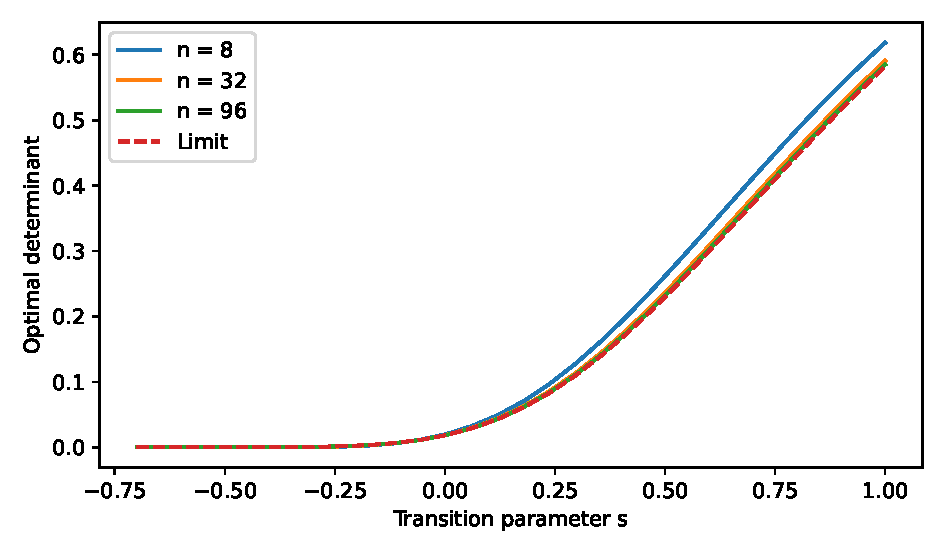
\includegraphics[width=.88\textwidth]{verification/determinant_transition.pdf}
 \caption{Numerically optimized determinants at
 $L=(n-1)(\frac12\log n+s)$ compared with the proved limit
 $\exp(-4e^{-2s})$. Curves are numerical diagnostics; the proof of convergence
 is independent of the optimization code.}
 \label{fig:transition}
\end{figure}

\section{Reproducible checks and numerical evidence}
\label{sec:numerics}

\subsection{Verification protocol}
The archive contains \texttt{verify.py}, its recorded output, machine-readable
JSON and CSV tables, and the two figures. The program has no network
dependency. The recorded environment was Python 3.13.5, NumPy 2.3.5,
SciPy 1.17.0, mpmath 1.3.0, and SymPy 1.14.0.
To reproduce the computations and regenerate the figures, run
\begin{verbatim}
python verify.py --output verification --figures
\end{verbatim}
% ed. (2026-09-29): editorial note added by ProveIt (changed rerun
% behaviour of verify.py, regenerated figures); not part of the delivered text.
\begin{quote}\small
\textbf{Editorial note (ProveIt, 2026-09-29).} In the filed package,
\texttt{verify.py} writes by default into a scratch directory
\texttt{verification\_rerun/}; writing into the recorded
\texttt{verification/} directory, as the command above does, also needs
\texttt{-{}-overwrite-recorded}, because a rerun on another platform changes
the last digits of the double-precision values recorded there. The two
figures were regenerated with TrueType instead of Type~3 fonts, from the same
code and data, and the requirements are pinned to the recorded versions
(Matplotlib 3.10.8, which wrote the delivered figures).
\end{quote}
The program performs exact rational coefficient checks with SymPy,
80-decimal-digit quadrature and small-dimensional Newton calculations with
mpmath, and double-precision convex optimization for larger designs.
The latter uses the exact analytic gradient and Hessian with a line search;
endpoints are fixed. No random samples enter these checks.

The checks address several independent parts of the argument: normalization
and constant potential; the elliptic-series coefficients; inverse-capacity
coefficients; eta modularity and the exact finite-product tail; the finite
Jensen enclosure; the dilute energy and gap corrections; and the
critical-window expansion. All programmed assertions passed in the
recorded run. The mpmath results are high-precision numerical diagnostics,
not rigorous enclosures, and the code is not a formal proof checker.

\subsection{Equilibrium normalization and potential}
The substitution $t^2=1+(b^2-1)\sin^2\theta$ removes the square-root
endpoint singularities from normalization. For the potential, the
integration interval is also split at its logarithmic singularity.
At $L=0.2,1,3$, normalization discrepancies were below $10^{-77}$ and
potential discrepancies at $u/L=0.1,0.5,0.9$ were below $10^{-79}$ at the
working precision. A displayed zero in the raw output means zero after
finite-precision rounding, not an exact symbolic integration certificate.
The equilibrium energies are
\begin{center}
\begin{tabular}{@{}rr@{}}
\toprule
$L$ & $I_L$\\
\midrule
$0.2$ & $2.99904551559535685251$\\
$1$ & $1.45927489567825624541$\\
$3$ & $0.66810270286063430161$\\
\bottomrule
\end{tabular}
\end{center}

For comparison, the fixed-interval minimizing energies at $L=1$ are:
\begin{center}
\begin{tabular}{@{}rr@{}}
\toprule
$n$ & $2E_n^*(1)/(n(n-1))$ (numerical)\\
\midrule
8 & 1.070740746589\\
16 & 1.232683639463\\
32 & 1.327711901636\\
64 & 1.383689948640\\
128 & 1.416371676477\\
\bottomrule
\end{tabular}
\end{center}
The convergence is visibly slower than the dilute critical-window
convergence. The table does not supply a rate for
\cref{thm:convergence}, and it would be inappropriate to infer the first
edge gap from these energy values.

\subsection{A direct test of the boundary energy gain}
Define the scaled grid-to-optimum gain
\begin{equation}
 G_{n,h}=e^{6h}\bigl(U_n(h)-E_n^*((n-1)h)\bigr).
 \label{eq:Gcheck}
\end{equation}
The theorem predicts $G_{n,h}\to2(n-3)/(n-1)$ for each $n$, with an error
bounded by an absolute constant times $e^{-2h}$ uniformly in $n$.
The 80-digit calculations give:
\begin{center}
\begin{tabular}{@{}rrrr@{}}
\toprule
$n$ & $G_{n,3}$ & $G_{n,4}$ & Predicted limit\\
\midrule
4 & 0.666287327830 & 0.666616746258 & 0.666666666667\\
8 & 1.435241666559 & 1.429474991882 & 1.428571428571\\
16 & 1.743372444134 & 1.734691207867 & 1.733333333333\\
\bottomrule
\end{tabular}
\end{center}
The raw file also records the energy error divided by $q^4$ and the
Euclidean gap error divided by $q^2$. Those quantities stay of ordinary
size in the tested cases, as predicted. Finite tests cannot establish
uniformity over all dimensions; that is supplied by the proof in
\cref{sec:boundary}.

\subsection{The critical window}
At $s=0$, let
$E_n^{(3)}=2-4/(3n^2)-20/(3n^3)$.
The following values test the three-order approximation:
\begin{center}
\begin{tabular}{@{}rrrr@{}}
\toprule
$n$ & Optimized $E_n$ & $\Dopt_n$ & $n^4(E_n-E_n^{(3)})$\\
\midrule
8 & 1.964989270450 & 0.019644094093 & $-4.73728$\\
16 & 1.993072791619 & 0.018571157326 & $-5.98153$\\
32 & 1.998488269347 & 0.018371099313 & $-6.49781$\\
64 & 1.999648646953 & 0.018328513923 & $-6.72596$\\
128 & 1.999915415425 & 0.018318737592 & $-6.83227$\\
\bottomrule
\end{tabular}
\end{center}
The limiting determinant is $e^{-4}=0.0183156388887\ldots$.
The last column is consistent with an $O(n^{-4})$ error but is not used
to guess or assert the next exact coefficient. The recorded stationarity
residuals for these critical-window optimizations range from about
$3.1\times10^{-13}$ to $3.6\times10^{-15}$.

\subsection{Product and inverse checks}
The direct and modular bulk formulas were compared at
$h=0.2,0.5,1,2$. Their discrepancies were below $10^{-79}$ at 80-digit
precision. The identity $U_n=nS-T+R_n$ was checked at the same values
with $n=9$, also below $10^{-78}$.
Exact symbolic calculations reproduce the first five coefficients of
$B(z)$, the first five coefficients in \eqref{eq:inverseexpansion}, and
the full polynomial in \eqref{eq:criticalenergy}. An additional inverse
check evaluates \eqref{eq:inverseexpansion} at the exact elliptic energies
for $L=1,2,3$; its residual divided by $Q^6$ approaches the next coefficient
$-4$, which is obtained from \eqref{eq:inversecoeff} rather than fitted
from the data.

\section{What remains open and a proposed research program}
\label{sec:questions}

The following questions are deliberately separated from the proved results.
They range from concrete extensions of the present estimates to more
structural transseries and formalization projects.

\subsection{Microscopic fixed-interval endpoint spacings}
\begin{question}
For fixed $L>0$ and fixed $j\ge1$, determine the limit, if it exists, of
$n^2u_{j+1}^{(n)}$, with $u_1^{(n)}=0$. Obtain the reflected right-edge law
and a transition to the bulk spacing scale.
\end{question}
The density coefficient in \eqref{eq:edge-density} identifies the natural
edge scale but not the discrete constant. A promising approach is to
rewrite \eqref{eq:stationarity} using $t_i=e^{2u_i}$, derive an equation
for the node polynomial or its logarithmic derivative, and study the
endpoint boundary layer. A proof would complete the endpoint portion of
\texttt{question:design-limit}; that portion is not settled here.

\subsection{The finite-density surface energy}
\begin{question}
For each fixed $h>0$, does
\[
 \Sigma(h)=\lim_{n\to\infty}
 \left(E_n^*((n-1)h)-nS(h)\right)
\]
exist? Can it be represented by a uniquely minimizing semi-infinite
boundary profile and an explicit correction for the fixed total length?
\end{question}
The bounds in \cref{thm:bounds} place the expression in a compact interval,
but boundedness alone does not prove a limit. The equal-grid contribution
is $-T(h)$. Any additional term measures boundary relaxation. An
existence proof should control how the two edge layers communicate through
the length constraint, not merely invoke exponential decay of pair forces.

\subsection{Higher uniform dilute coefficients}
\begin{question}
Develop, for every fixed $N$, a dimension-uniform expansion of the optimal
gap vector and energy through $q^N$. Determine which coefficients stabilize
as $n\to\infty$, and isolate the rational $1/(n-1)$ corrections caused by
the zero-sum projection.
\end{question}
The uniformly contractive representation in \cref{lem:local} provides a
starting point. The challenge is to preserve an absolute energy remainder
rather than an $n$-dependent bound at each order. The $q^4$ surface
coefficient would immediately determine the $n^{-4}$ critical-window
coefficient. The numerical table is useful as a regression test, but
coefficient identities should be derived symbolically.

\subsection{A mesoscopic bridge between elliptic and crystalline limits}
\begin{question}
Find uniform asymptotics when $L=L_n\to\infty$ but $h_n=L_n/(n-1)\to0$.
Which subregimes permit the fixed-interval elliptic energy to match the
small-$h$ expansion of $nS(h)$, and where do entropy-like discrete
corrections first change the answer?
\end{question}
The fixed-$L$ theorem and the positive-gap theorem cannot be interchanged
without proof. Formally, $I_L\sim\pi^2/(4L)$ and
$S(h)\sim\pi^2/(8h)$ yield matching leading energies
$\pi^2n^2/(8L)$, but the next orders contain different boundary and
discreteness information. A uniform comparison would connect the elliptic
and modular transseries in a genuinely two-parameter theorem.

\subsection{The full hyperbolic superfactorial crossover}
\begin{question}
Starting from \eqref{eq:finiteproductexact}, determine a complete joint
asymptotic as $h\downarrow0$ and $n\to\infty$, uniformly in prescribed
ranges of $nh$. Include the MacMahon surface contribution and the exact
finite-size tail at the same precision.
\end{question}
The exact factorization solves an algebraic part of the repository's
\texttt{question:q-barnes}, but not its full asymptotic request.
A Mellin representation of $\log M(e^{-t})$ is a natural route to
power-logarithmic terms; a further analysis is needed to justify optimal
truncation and exponentially small corrections. The convergent eta
expansion for $S$ is not a substitute for that analysis.

\subsection{General screened logarithmic interactions}
\begin{question}
Suppose $W$ is decreasing, strictly convex, logarithmically singular at
zero, and has a convergent large-distance expansion
$W(x)=c_1e^{-\alpha x}+c_2e^{-2\alpha x}+\cdots$, with $c_1>0$.
Which hypotheses give a dimension-uniform boundary correction analogous
to \cref{thm:boundary}, and which coefficients determine its first term?
\end{question}
The Jensen certificates and bounded-defect argument use much less than
the special hyperbolic form. The projected grid force and Hessian method
suggest a general theorem for sufficiently controlled exponential tails.
One should distinguish the universal boundary mechanism from the exact
elliptic equilibrium and determinant identities, which are special here.

\subsection{Several allowed intervals and external fields}
\begin{question}
Determine equilibrium measures when the admissible $u$-set is a union of
intervals, or when the objective includes a smooth external field. Can
one classify support transitions and produce uniform expansions near a
newly opening or closing support component?
\end{question}
Under $t=e^{2u}$, the one-interval calculation becomes an arcsine Cauchy
integral. Several intervals lead to a more complicated algebraic
singular-integral problem with unknown filling fractions. This offers a
concrete setting for multi-scale inversion and critical transseries,
but no multi-interval formula is claimed in the present paper.

\subsection{Covariance spectrum beyond the determinant}
\begin{question}
At the optimal configurations, determine the smallest eigenvalue,
condition number, and empirical eigenvalue distribution of
$[\sech(u_i-u_j)]$. How do they behave in the fixed-$L$, positive-gap,
and dilute critical regimes?
\end{question}
A determinant is only the product of eigenvalues. The limit
\eqref{eq:maintransition} alone does not yield a lower bound on every
eigenvalue or establish numerical stability of interpolation. The
Cauchy-matrix representation may permit explicit inverse formulas and
more refined spectral estimates.

\subsection{Sharp nonasymptotic numerical certification}
\begin{question}
Combine interval arithmetic, convexity, and the explicit Hessian with
\eqref{eq:bracket} to produce rigorous finite-$n$ enclosures of the true
optimizer, its determinant, and its edge gaps. Can the certified cost
be reduced below dense cubic-time Newton solves?
\end{question}
The supplied code is a transparent diagnostic, not a complexity-optimized
solver. The covariance Cauchy structure and exponentially decaying
interactions suggest structured linear algebra or certified truncation,
with distinct choices in dense and dilute regimes.

\subsection{Formal proof of the finite-dimensional core}
\begin{question}
Formalize the determinant identity, Jensen enclosure, and projected
boundary estimates in Lean, and then connect them to a formalized
measure-theoretic equilibrium theorem.
\end{question}
The finite inequalities are natural first milestones: they avoid
principal-value integration and elliptic special functions while already
providing useful certified determinant estimates. A later stage should
formalize the arcsine integral and its endpoint continuity, rather than
introducing the whole equilibrium theorem as an axiom.

\section{Formalization boundary and proof dependency map}
\label{sec:formalization}

No Lean code is included or claimed to have compiled. The following
partition identifies what a future formalization would actually need.

\paragraph{Finite algebra and inequalities.}
The Cauchy determinant identity, geometric series, derivatives of $V$,
strict convexity, finite Jensen bounds, and the count $N_{i,k}$ are the
most self-contained layer. The main dependencies are finite sums,
matrices, elementary real analysis, and constrained convex optimization.
The dimension-free window bounds require estimates uniform in a natural
number parameter, not an infinite-dimensional optimizer.

\paragraph{Analytic fixed-point layer.}
The projected contraction and its sup/Euclidean norm conversion establish
\cref{thm:boundary}. A formal proof should expose the constants and a
permitted $q_0$, instead of hiding them in successive uses of $O(q)$.
The manuscript's existence of absolute constants follows from explicit
convergent majorant sums; it does not yet provide a machine-readable
optimized numerical threshold.

\paragraph{Measure and special-function layer.}
The continuum proof requires logarithmic-potential continuity,
principal-value differentiation, a Fourier positivity argument for finite
signed measures, and weak compactness. The elliptic definitions are
ordinary real integrals. The capacity transseries then adds the standard
elliptic expansion, while the bulk modular transseries adds the eta
transformation. These are logically separate inputs.

\paragraph{Dependency summary.}
The chain for the new finite-size result is
\[
 \text{window counting}\ \Longrightarrow\
 \text{localized grid force}\ \Longrightarrow\
 \text{uniform projected contraction}
\]
\[
 \Longrightarrow\ \text{Euclidean Hessian control}\
 \Longrightarrow\ \text{boundary energy correction}
\]
\[
 \Longrightarrow\ \text{critical-window expansion}.
\]
It does not depend on the continuum equilibrium theorem or on elliptic
or modular special-function identities. Conversely, the fixed-$L$
equilibrium theorem is independent of the dilute expansion. This
separation gives independent audit targets and prevents a numerical
check of one regime from being misrepresented as evidence for another.

\section{Conclusion}
The fixed-interval design question from the Fabius report has an explicit
answer at the level of equilibrium measure and optimal leading energy.
Its density is \eqref{eq:main-density}, its constant potential is
\eqref{eq:main-I}, and its edge enhancement and screened bulk are described
by \cref{prop:edges,prop:continuumregimes}. These formulas connect the
repository to classical elliptic Green capacity in a precise normalization.
Their expansion and inversion supply convergent, quantitatively controlled
examples for the transseries program.

The finite-design problem has additional structure that the equilibrium
measure does not capture. The finite Jensen enclosure works for every
$n,L$; the positive-gap limit has bounded total gap defect; and the dilute
boundary correction is an absolute, dimension-uniform expansion. That
last point makes it possible to resolve the deterministic determinant
transition and calculate three finite-size correction orders without
replacing the optimum by an unjustified uniform-grid approximation.

The remaining questions are substantive. In particular, the fixed-interval
microscopic edge problem, the finite-density surface energy, and the full
joint MacMahon crossover are not hidden inside the results proved here.
They are explicit next targets with concrete formulas and verification
infrastructure on which to build.

\appendix
\section{Source provenance and reproducibility}
\label{sec:provenance}

The inspected repository is \texttt{VladimirReshetnikov/ProveIt}.
The source report's path is
\begin{quote}\small\raggedright
\path{Analysis/FabiusFunction/docs/semi-formalized-research-frontiers/drafts/representations/common_digit_fabius_zonoids_frontier_report/common_digit_fabius_zonoids.tex}.
\end{quote}
The repository search identified commit
\texttt{0c973d8f5e7ef4550f4df1bf486d890037fd9f14}; a direct read at that
commit confirmed the question block at source lines 1744--1785. The blob
identifier is \texttt{dabfc501dfe952d826001703a087b47424568581}.
The finite node-design statement was inspected in the same source's
1370--1590 range. The exact label of the primary question is
\texttt{question:design-limit}; the adjacent product question is
\texttt{question:q-barnes}. The source was accessed on 29 September 2026.

The transseries collection's README was also inspected to understand the
repository's current organization and its distinction between formalized
modules and unreviewed research arrivals. It was not used as evidence
that any theorem in this manuscript is formalized. No repository files
were modified during this work.

The archive contains the standalone source \texttt{article.tex}, the
compiled \texttt{article.pdf}, \texttt{verify.py}, the recorded
\texttt{verification.log}, tables and figure files under
\texttt{verification/}, and a short README and provenance file. The
article can be rebuilt with
\begin{verbatim}
pdflatex -interaction=nonstopmode -halt-on-error article.tex
pdflatex -interaction=nonstopmode -halt-on-error article.tex
pdflatex -interaction=nonstopmode -halt-on-error article.tex
\end{verbatim}
The supplied figure PDFs are sufficient for rebuilding; regenerating them
requires Matplotlib. Font files and third-party research PDFs are not
redistributed in the package.

\section{A convenient coefficient ledger}
\label{sec:ledger}
For exact regression testing, several derived quantities are collected
here with their independent definitions.

\begin{center}
\begin{tabular}{@{}rlll@{}}
\toprule
$j$ & $[z^j]B(z)$ & $[Q^j](L-X+\log2)$ & $c_j$ in \eqref{eq:Smodular}\\
\midrule
1 & $1/4$ & $2$ & $-1$\\
2 & $13/128$ & $-3$ & $1/2$\\
3 & $23/384$ & $8/3$ & $-4/3$\\
4 & $2701/65536$ & $-3/2$ & $5/4$\\
5 & $5057/163840$ & $12/5$ & $-6/5$\\
\bottomrule
\end{tabular}
\end{center}
The two occurrences of $Q$ in this ledger belong to different problems:
for inverse capacity, $Q=e^{-\pi^2/I}$; for the bulk energy,
$Q=e^{-\pi^2/h}$. They are not being identified. The first column is
obtained from $B=D/A$, the second from \eqref{eq:inversecoeff}, and the
third from divisor sums. All entries are exact rational numbers.

The critical-window energy coefficients, in powers of $1/n$, are
\begin{align*}
 C_0(a)&=2a,\\
 C_1(a)&=2a^2-2a,\\
 C_2(a)&=\tfrac83a^3-4a^2,\\
 C_3(a)&=2a^4-\tfrac{26}3a^3.
\end{align*}
In particular, the boundary relaxation contributes exactly $-2a^3$ to
$C_3$, and no contribution to $C_0,C_1,C_2$. This is a useful normalization
check: accidentally using the product energy in place of the log
determinant would change every final logarithmic coefficient by a factor
of two.

\begin{thebibliography}{9}
\bibitem{repo}
VladimirReshetnikov/ProveIt repository,
\emph{Common-Digit Fabius Zonoids: Exact volumes, hyperbolic-secant geometry,
Bernoulli Gaussianization, and parameter jets}, research report,
commit \texttt{0c973d8f5e7ef4550f4df1bf486d890037fd9f14}.
The source path and question labels are recorded in
\cref{sec:provenance}. Accessed 29 September 2026.
\url{https://github.com/VladimirReshetnikov/ProveIt}.

\bibitem{saff}
E.~B. Saff,
\emph{Logarithmic Potential Theory with Applications to Approximation Theory},
Surveys in Approximation Theory \textbf{5} (2010), 165--200.
\url{https://arxiv.org/abs/1010.3760}.

\bibitem{nrv}
M.~M.~S. Nasser, O. Rainio, and M. Vuorinen,
\emph{Condenser capacity and hyperbolic diameter},
Journal of Mathematical Analysis and Applications,
DOI: \href{https://doi.org/10.1016/j.jmaa.2021.125870}{10.1016/j.jmaa.2021.125870}.
Inspected version: arXiv:2011.06293v2, 27 November 2021,
especially the elliptic capacity formulas in Section 2.
\url{https://arxiv.org/abs/2011.06293}.

\bibitem{dlmf19}
NIST Digital Library of Mathematical Functions,
Chapter 19, \S19.12, \emph{Asymptotic Approximations},
particularly formulas 19.12.1 and 19.12.3 for the convergent expansion of
$\K$ near complementary modulus zero. Accessed 29 September 2026.
\url{https://dlmf.nist.gov/19.12}.

\bibitem{dlmf23}
NIST Digital Library of Mathematical Functions,
Chapter 23, \S23.18, \emph{Modular Transformations},
particularly the Dedekind eta transformation, formula 23.18.5.
Accessed 29 September 2026.
\url{https://dlmf.nist.gov/23.18}.
\end{thebibliography}
\end{document}
